% Titre de la premiere partie
\section{Introduction Historique}

%%%%%%%%%%%%%%%%%%%%%%%%%%%%%%%%%%%%%%%%%%%%%%%%
% Première diapo
%%%%%%%%%%%%%%%%%%%%%%%%%%%%%%%%%%%%%%%%%%%%%%%%
\begin{frame}
\frametitle{Introduction historique}
\framesubtitle{Position du problème}

\begin{itemize}
	\item	<1->	La mécanique newtonienne, une mécanique bien huilée
	\item	<2->	Précession du périhélie de Mercure
	
	\visible<3->{
	\begin{figure}
	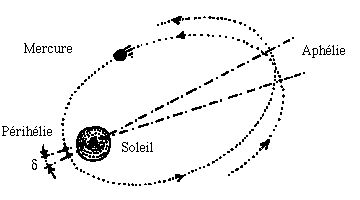
\includegraphics[width=0.8\linewidth]{figures/Fig01}
	\end{figure}
	}
	
\end{itemize}

\end{frame}


%%%%%%%%%%%%%%%%%%%%%%%%%%%%%%%%%%%%%%%%%%%%%%%%
% Deuxième diapo
%%%%%%%%%%%%%%%%%%%%%%%%%%%%%%%%%%%%%%%%%%%%%%%%
\begin{frame}
\frametitle{Introduction historique}
\framesubtitle{Explication classique}

\begin{itemize}
	\item	<1->	Théorie des perturbations: explication de $531''$ d'arc/siècle
	\item	<2->	Vulcain, un bon candidat (Le Verrier, 1859)
	\item	<3->	mais pas de confirmation expérimentale...
	
\end{itemize}

\end{frame}


%%%%%%%%%%%%%%%%%%%%%%%%%%%%%%%%%%%%%%%%%%%%%%%%
% Troisième diapo
%%%%%%%%%%%%%%%%%%%%%%%%%%%%%%%%%%%%%%%%%%%%%%%%
\begin{frame}
\frametitle{Introduction historique}
\framesubtitle{Complément relativiste}

\begin{itemize}
	\item	<1->	La relativité restreinte permet déjà un mieux ($7''$ d'arc 
	en plus par siècle)

	\item	<2->	mais c'est la générale qui va sauver la mise en ajoutant 
	les $43''$ qui manquaient
	
\end{itemize}

\end{frame}
